\documentclass{article}

\usepackage{graphicx, xcolor}
\usepackage{amsmath, amssymb}
\usepackage[colorlinks=true,allcolors=blue]{hyperref}

\usepackage[margin=1in]{geometry}

\def\hwtitle{Homework 3: Ordinary Differential Equations, Part 1}
\def\hwauthor{Caden Gobat}
\def\hwdate{\today}

\usepackage{fancyhdr}
\lhead{\hwauthor}
\chead{\hwtitle}
\rhead{\hwdate}
\lfoot{\hwauthor}
\cfoot{}
\rfoot{\thepage}
\renewcommand{\footrulewidth}{0.4pt}
\pagestyle{fancy}

\author{\hwauthor}
\title{\hwtitle}
\date{\hwdate}

\begin{document}

\maketitle
\thispagestyle{fancy}

\section{Introduction}

Last week we explored some simple integration techniques for evaluating ODEs numerically.

\section{Results}

\bigskip
\noindent{\bf Question 1}
\medskip

\begin{itemize}
    \item $GM_\odot$ in ``Earth orbit'' units (AU and years) has a numerical value of $(2\pi)^2=4\pi^2\approx39.4784$
    \item Earth must travel a distance of $2\pi(1 \text{ AU})$ in a year. Thus its tangential velocity is simply $2\pi\ \frac{\text{AU}}{\text{year}}$.
\end{itemize}

\bigskip
\noindent{\bf Question 2}
\medskip

\begin{figure}[h!]
    \centering
    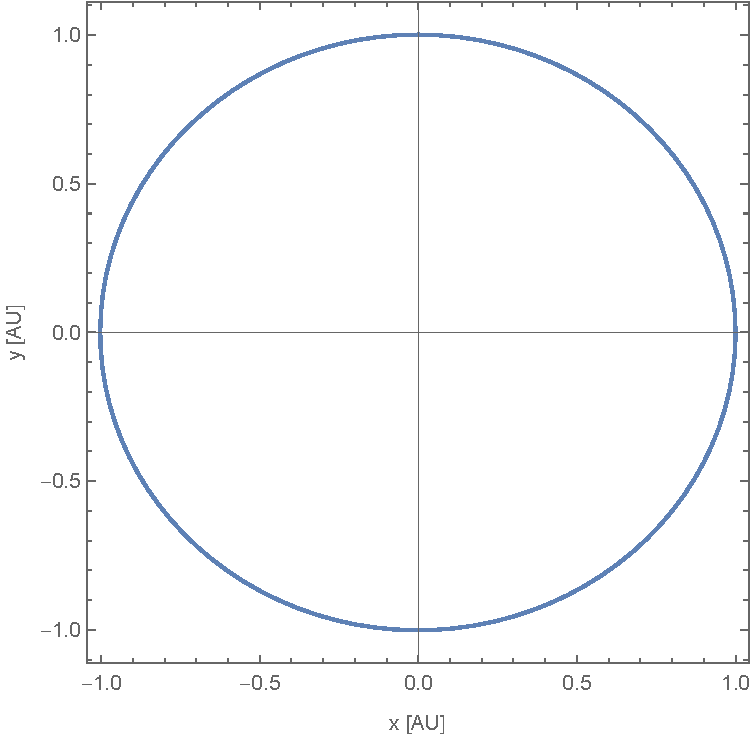
\includegraphics[width=3.5in]{homework3/q2_orbit.pdf}
    \caption{Using the initial conditions discussed in \textbf{Question 1}, we can simulate an orbit for the Earth that is approximately circular over the course of a year.}
    \label{fig:q2orbit}
\end{figure}

\begin{figure}[h!]
    \centering
    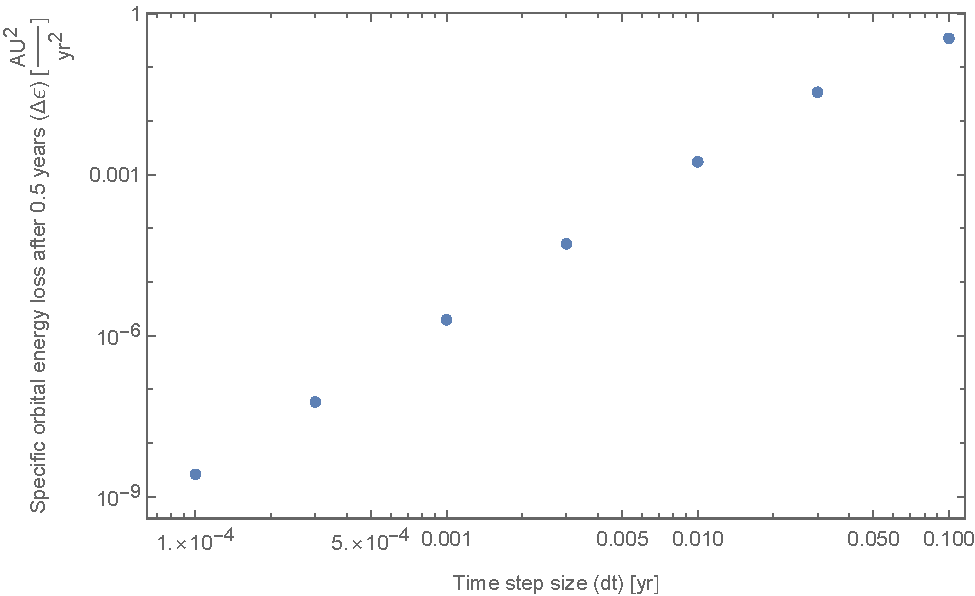
\includegraphics[width=5in]{homework3/q2_energyloss.pdf}
    \caption{Log slope is approximately 2.781}
    \label{fig:q2energy}
\end{figure}

\bigskip
\noindent{\bf Question 3}
\medskip

\begin{figure}[h!]
    \centering
    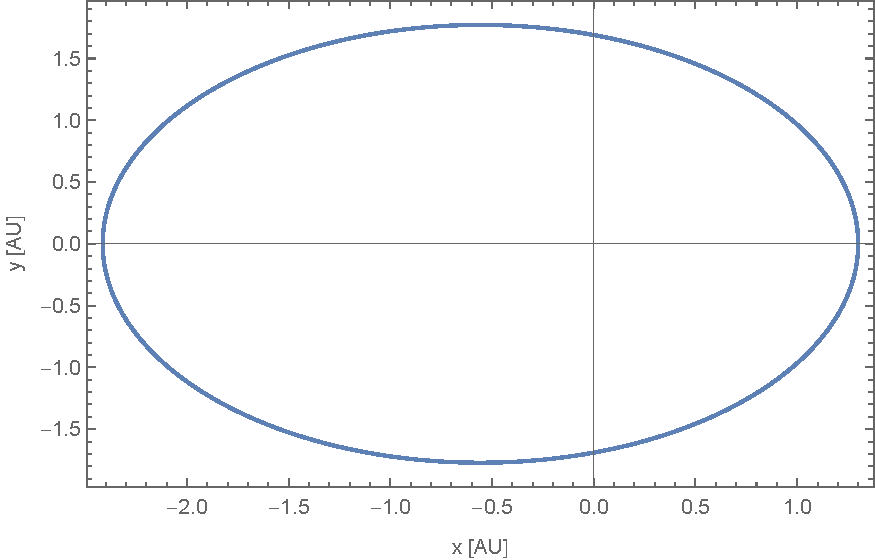
\includegraphics[width=5in]{homework3/q3_orbit.pdf}
    \caption{Trajectory of an eccentric orbit using $(x_0,y_0)=(1.3,0)$; $(v_{x,0},v_{y,0}=(0,2\pi)$; and $dt=0.001$ yr.}
    \label{fig:q3orbit}
\end{figure}

This orbiting body starts at perihelion, or $R_\text{min}$, 1.3 AU. It reaches a maximum distance (aphelion) of 2.414 AU, meaning the ratio is $\frac{r_a}{r_p}=1.857$

\begin{figure}[h!]
    \centering
    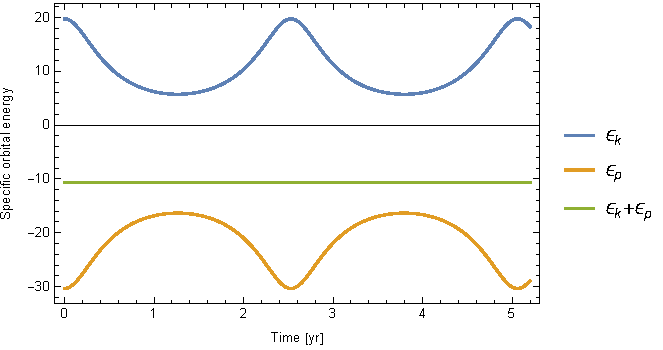
\includegraphics[width=5in]{homework3/q3energy.pdf}
    \caption{Orbital energies per unit mass, plotted over two complete periods. As expected, the total energy remains nearly constant, with potential and kinetic being converted back and forth into one another throughout the orbit.}
    \label{fig:q3energy}
\end{figure}

\bigskip
\noindent{\bf Question 4}
\medskip

\begin{figure}[h!]
    \centering
    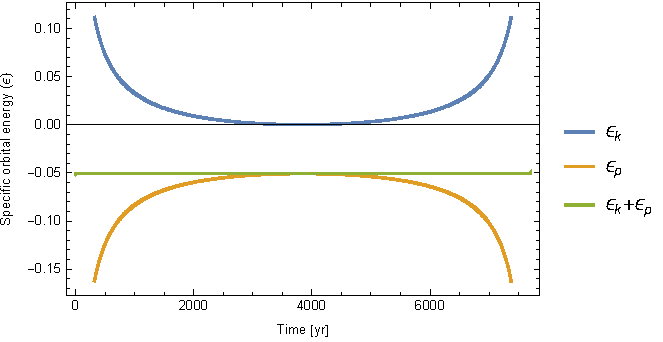
\includegraphics[width=5in]{homework3/q4energy.pdf}
    \caption{Caption}
    \label{fig:q4energy}
\end{figure}

\section{Conclusions}

These exercises demonstrated both the power and the limitations of numerical integration techniques. A multitude of factors go into determining the accuracy with which a numerical integrator can be used, such as algorithm, step size, domain range, type of integrand, and even initial (starting) conditions.

We saw that for an exponential, the order of convergence for midpoint summation goes as $h^2$, whereas that of lefthand summation is linear in $h$. The most challenging piece of this assignment for me personally was understanding this kind of pseudo big-$\mathcal{O}$ notation to talk about the rates at which different algorithms converge to the analytical solution.

In all, this assignment went well and I came away with a better understanding of how to implement numerical methods in C.

\end{document}
